\chapter{前言}
\renewcommand{\baselinestretch}{10.0} %設定行距
\pagenumbering{arabic} %設定頁號阿拉伯數字
\setcounter{page}{1}  %設定頁數
\fontsize{14pt}{2.5pt}\sectionef
\section{作業內容}
協同產品設計實習的 Project 1 目的是讓學員可以從 \\
https://mde.tw/cd2023/content/BubbleRob.html 導引練習中, 了解 CoppeliaSim 套件中的諸多功能以及用法, 其中包括利用近接感測器偵測障礙物, 並透過 Lua script 控制 bubbleRob 雙輪車的移動. 為了讓各組學員了解在多人協同模式下, 開發機電資產品流程中必須面臨的許多議題(若要直接在瀏覽器中建立多方協同的場景, 可以透過 remote API(導引) 與 Visualization Stream 功能).自 W5 起將建立一個由 pj1 各組組長所組成的統整作業, 目標是利用兩台 BubbleRob 雙輪車在一足球場景中進行對戰, 其中在雙方球門設置感測器, 雙方各有一名 BubbleRob 負責運球, 在規定時間內, 每進一球後, 即透過程式重新從球場中線發球重啟賽局. 其中各組必須設法配置計分板顯示比賽剩餘時間與比分。\\

\begin{figure}[hbt!]
\begin{center}
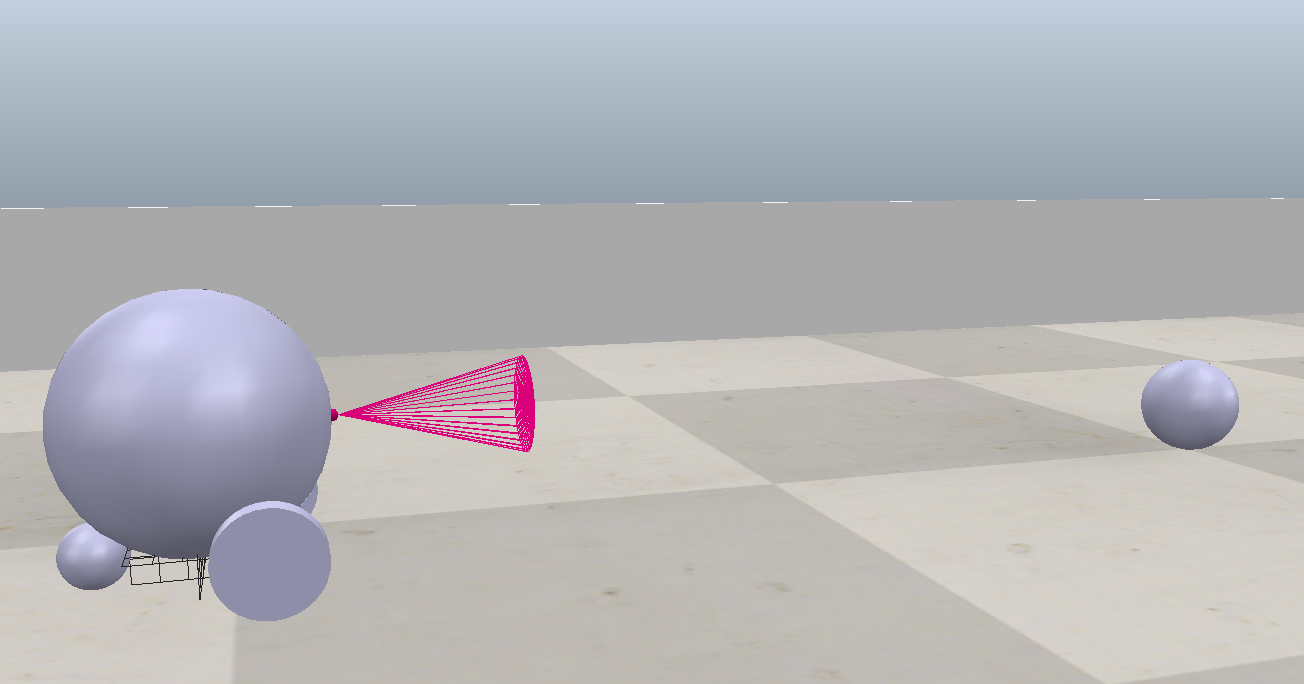
\includegraphics[width=15cm]{車車}
\caption{\Large 泡泡機器人主體 }
\label{泡泡機器人主體}
\end{center}
\end{figure}


\section{遊戲規則}
遊戲規則如下:\\

Pong game 的遊戲規則簡單,透過bubbleRob將球打入對方球門即得一分,時間內其中一方分數最高即可獲勝,當有一方滿五分時遊戲結束。
\\
\\
\\
\\
   
\begin{figure}[hbt!]
\begin{center}
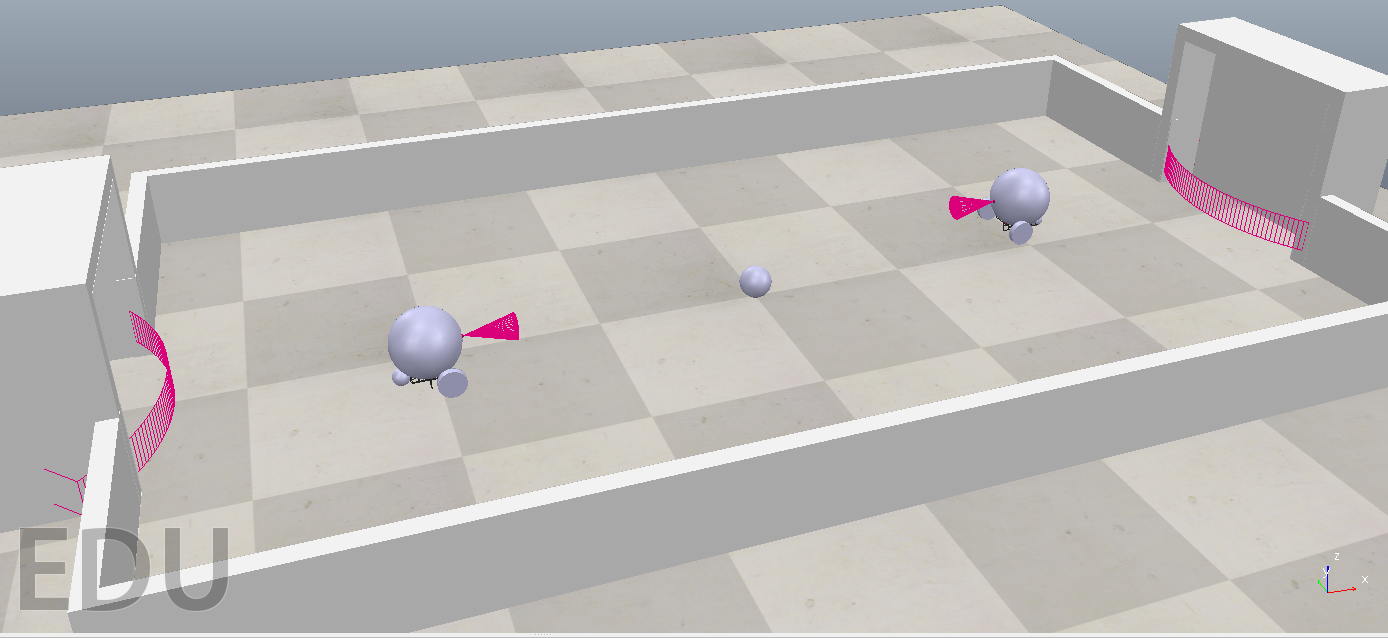
\includegraphics[width=15cm]{兩車車}
\caption{\Large 主體和場地}
\label{主體和場地 }
\end{center}
\end{figure}
\newpage


